%% LyX 2.0.6 created this file.  For more info, see http://www.lyx.org/.
%% Do not edit unless you really know what you are doing.
\documentclass[english]{article}
\usepackage[T1]{fontenc}
\usepackage[utf8]{luainputenc}
\usepackage{graphicx}
\usepackage{amsmath}
\usepackage{babel}
\begin{document}

\title{Analysis of 2012 and 2014  Beamtests }

\maketitle

\section{Event selection}


\section{Time analysis}


\section{Seed Analysis}


\subsection{Hits tagging}

Hits are separated in 3 categories:
\begin{itemize}
\item ISOLATED= The hit has no neighbours in a 6 cm radius sphere
\item EDGE = The hit belongs to a track segment in a 6 cm radius sphere
\item CORE= all other hits
\end{itemize}
Each hit defines a neighbouring sphere of 6 cm and a principal component
anlysis is done on all neighbours. The ratio w of the 2 principal
axis is then used to tag the hit.
\begin{itemize}
\item w=0 $\rightarrow$ less than 3 neighbours, the hit is ISOLATED
\item w < 0.3  $\rightarrow$ the second axis is small, most probably hits are aligned
along the first axis, the hit is an EDGE one.
\item w > 0.3 , the hit is in the CORE of the shower.
\end{itemize}
The figure \ref{fig:Ratio-of-L2/L1} shows the distribution of w for
all the hits of a 60 GeV pion run. The 3 categories clearly exhibits.
On figure \ref{fig:Ratio-of-L2/L1-track} the same ratio is shown
for preselected muon candidates and preselected pions interaction
in the same run.

\begin{figure}
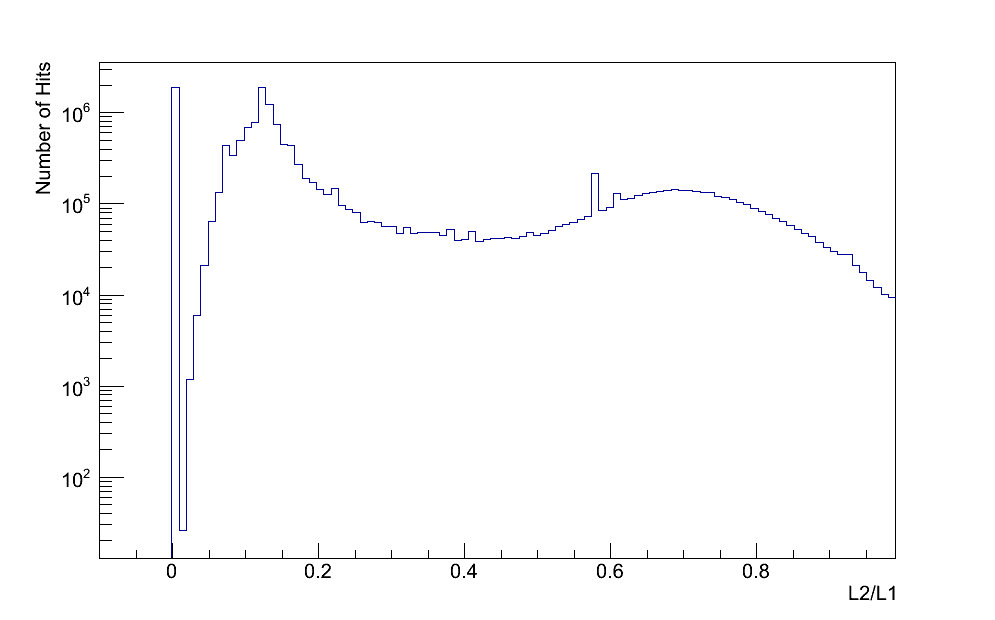
\includegraphics[width=1\textwidth]{Hits_Weight}

\caption{\label{fig:Ratio-of-L2/L1}Ratio of L2/L1 derived from PCA of neighbours
hits}


\end{figure}


\begin{figure}


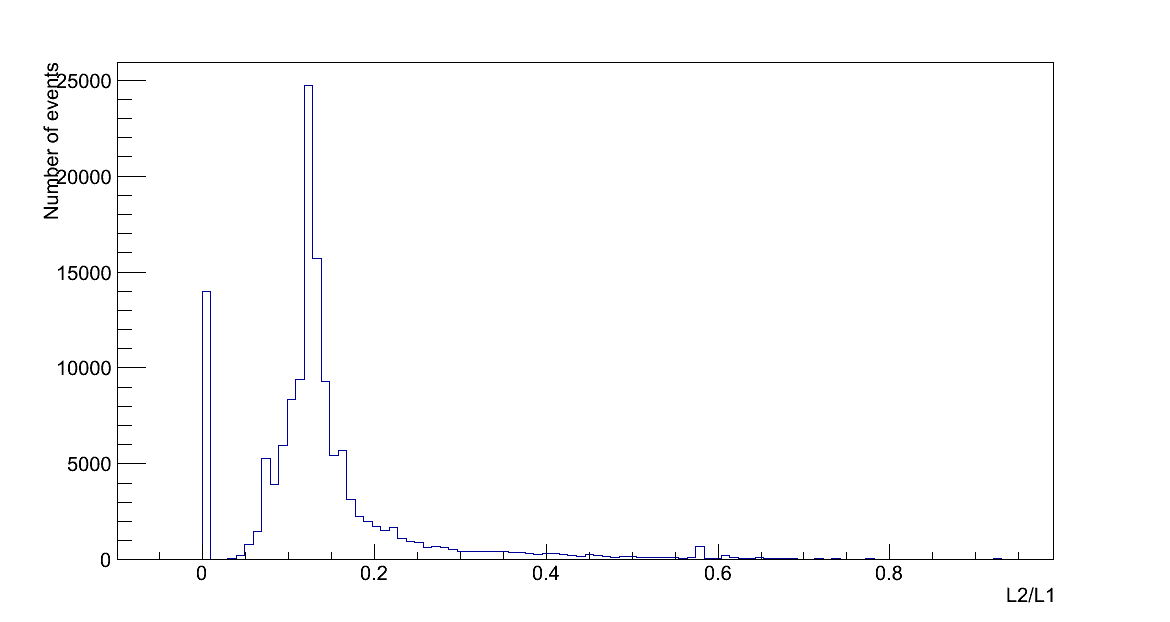
\includegraphics[width=1\textwidth]{Hits_Weight_track}

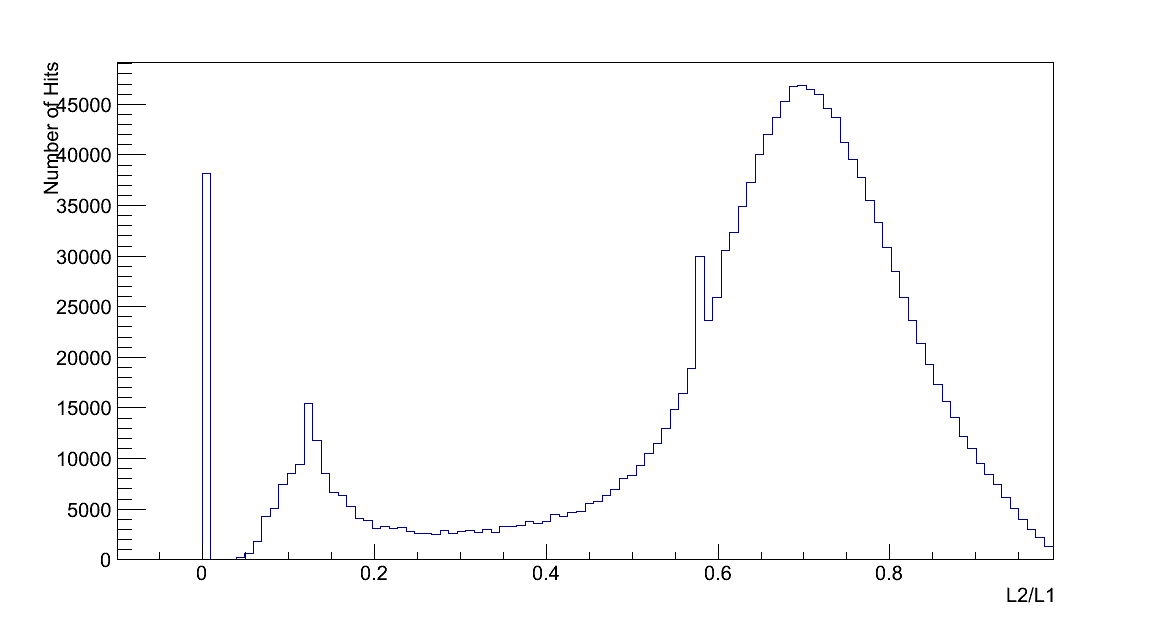
\includegraphics[width=1\textwidth]{Hits_Weight_shower}\caption{\label{fig:Ratio-of-L2/L1-track}Ratio of L2/L1 for preselected muon
tracks (top) and preselected showers (bottom) }
\end{figure}



\subsection{MIP tagging}

Once hits are sorted in those three categories. Clusters are built
plane by plane by adding hits in plane distant from less than 4 cm
to an existing cluster. Two collections are built. ``Interaction''
clusters are built from CORE hits and ``real'' clusters from the
other hits. Finally ``Interaction'' clusters of less than 5 hits
are moved in the ``real'' collection and in paralell ``real''
clusters of more than 5 hits are moved in the ``interaction'' one.

The ``real'' collection is then used to reconstructed track segments
according to this algorithm:
\begin{itemize}
\item Once again a principal component anlysis is used for all clusters to
find main direction in a 15 cm sphere around each point
\item Each point is associated to existing tracks according to:

\begin{itemize}
\item if the track has at least 2 hits, the error of the extrapolation is
taken and the point is added if

\begin{itemize}
\item It is not the track path
\item it is less than 3 planes away from the end of the track
\item it is less than 5 sigma from the extrapolation
\end{itemize}
\item if the track has only one hit

\begin{itemize}
\item the track hit is one plane before
\item the principal axis of the cluster is used to build track parameter
and point is added if it is less than 6 cm from the extrapolation
\end{itemize}
\end{itemize}
\item If no association is found, a new single hit track is created with
track parameters deduced from the principal component analysis of
its neighbouring.
\end{itemize}
The algorithm is run handling hits from the beam entry to the end
of the calorimeter. At the end , a last pass is done trying to associate
single hit tracks and previously unselected hits to valid segments.
Finally all hits belonging to a cluster associated to a track segment
are tagged MIP. The figure \ref{fig:60-GeV-Pion} shows the result
of the different steps of the algorithm.

\begin{figure}
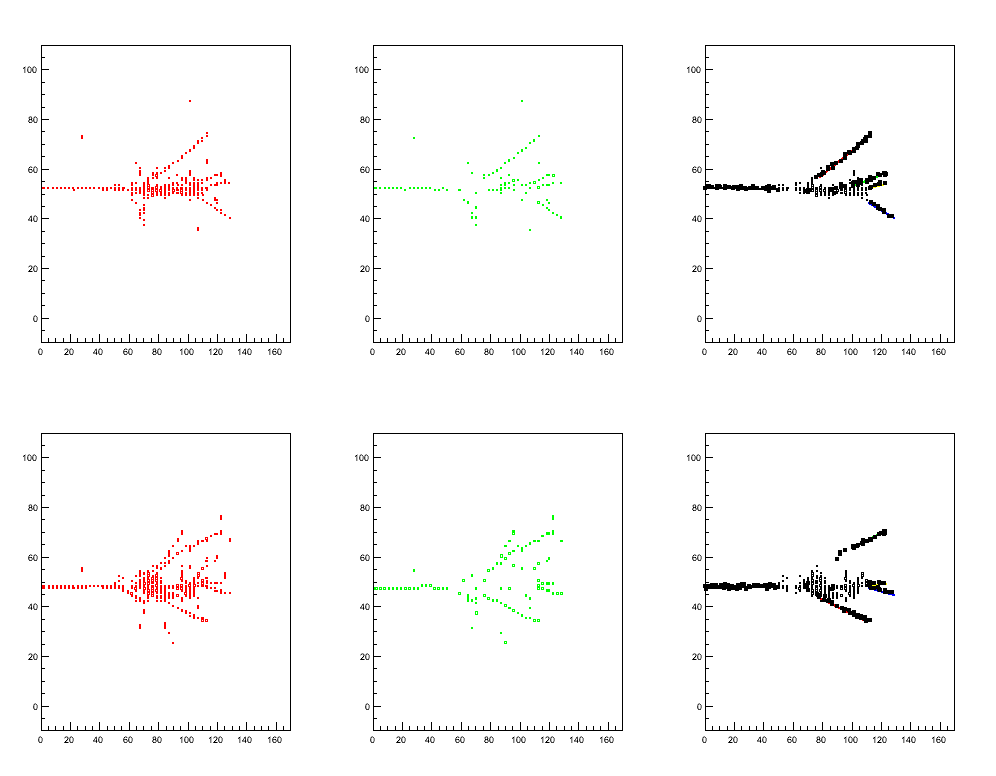
\includegraphics[width=1\textwidth]{60GevPion_MIP}

\caption{\label{fig:60-GeV-Pion}60 GeV Pion interaction display. The left
(red) column shows the hits position in (Z,X) and (Z,Y) projection.
The midle (green) column shows the ``real'' collection of clusters
projection. Finally on the right, track segments, MIP hits (black)
and 3D clusters of CORE hits are shown}
\end{figure}


The track segments can also be used to dicriminate muons and elctrons
from hadrons, using the ration of the total track length over the
total number of hits. The figure \ref{fig:Ratio-of-LOH} shows this
ratio. The peak at zero corresponds to electron with no MIP exiting
from the shower. The 1.4 peak is due to muons with a hit multiplicity
\textasciitilde{} 1.6 and finally hadron showers have a low ratio
up to 0.7. Events are tagged:
\begin{itemize}
\item ELECTRON if R<1E-4
\item MUON if R> 0.75
\end{itemize}
\begin{figure}
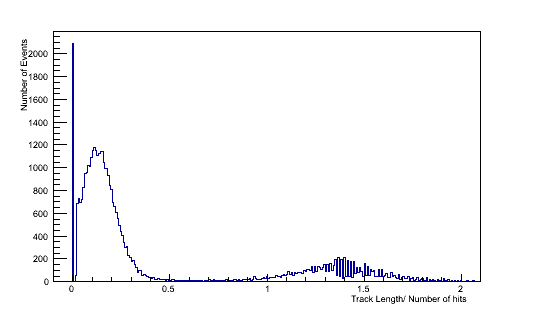
\includegraphics[width=1\textwidth]{TrackLength_Over_Hits}

\caption{\label{fig:Ratio-of-LOH}Ratio of total tracks length over the total
number of hits per event in a 60 Gev Pion run}


\end{figure}
\section{Shower Analysis}
\subsection{Shower building and selection}

Hits are grouped per plane. A loop on all planes starting from beam entry is run. An unassociated hit is the seed of a new "shower". A hit is associated to a shower if the distance of the hit to one hit of an exiting shower is 

 $$ D_{i,j} =  2 \times (  |I_i - I_j | + |J_i-J_j| ) + |plane_i-plane_j| < 15 $$
 
 
 A second pass is done once all hits are associated, merging showers when at least one of the first one hits is less than 20 distant from the second one.

Only showers with more than 4 planes are kept adn a principal analysis is run rejecting "muons" , ie, showers where $ \sqrt{\frac{l0+l1}{l2}} < 0.01 $  
 
 Events with more than one shower found are rejected for the energy and resolution analysis.
 
 This method is efficient to build the showers topology but rejected isolated hits or clusters (up to 10 \% of loss).  In the following analysis all hits in the calorimeter are considered and not only those included in the single selected one.   

\subsection{Shower selection}
 
 A final selection is done to remove interaction prior to the calorimeter
 $$ | x_{shower}- 50| < 15 ~ cm , ~ ~ | y_{shower} - 45| < 15 ~ cm$$
 
 Electron are rejected asking:
 
 $$ N_{MIP} \ne 0  ~ \& ~ Length(tracks) > 30 ~ cm $$
 
 Residuals muons are cut with
 
 $$  \frac{N_{MIP}}{N_{hits}} < 0.5 ~ \& ~  \frac{Length(tracks)}{N_{hits}}<0.5$$
 
 Finally to minimize leakage , the first interaction plane  is bellow 10, more than 5 interaction plane are required and more than 50 \% of the shower hitted planes should see an interaction ( An interaction plane is defined as a plane where more than 5 hits are seen  and the hits dispersion is bigger than 1.5 cm).
 
 \subsection{ Energy calibration}
 
 The shower energy is fitted to the following function:
 \begin{equation}
 \begin{split}
 E_{rec} = C \times ( Track_{length} \times (\alpha_{MIP} + \beta_{MIP} \times N_{hit}) \\ 
 + N_{0} \times (\alpha_{0} + \beta_{0} \times N_{hit}) \\
 + N_{1} \times (\alpha_{1} + \beta_{1} \times N_{hit} +\gamma_{1} \times N_{hit}^2 ) \\ 
 + N_{2} \times (\alpha_{2} + \beta_{2} \times N_{hit} +\gamma_{2} \times N_{hit}^2 )   
 \end{split}
 \end{equation}
 where $N_{0..2}$ is the number of hits for each threshold excluding the ones tagged MIP. Track length or number of MIP hits leads to the same energy resolution.
 December 2014  pions runs at 20,50 and 80 GeV are used and the Fit converged to:
 \begin{equation}
 \begin{split}
 C = 6.864E-02 \pm 5.334E-04  \\
\alpha_{MIP} = 9.041E-02 \pm 3.000E-02 \\
\beta_{MIP} = -1.508E-04 \pm 3.128E-05 \\
\alpha_0 = 7.816E-01 \pm 8.481E-03 \\
\beta_0  = 4.292E-07 \pm 7.603E-06 \\
\alpha_1 = 7.704E-01 \pm 3.123E-02 \\
\beta_1  = -3.201E-04 \pm 3.247E-05 \\
\gamma_1 = 3.643E-07 \pm 2.131E-08 \\
\alpha_2 = 1.407E-01 \pm 8.861E-02 \\
\beta_2  = 8.234E-03 \pm 1.039E-04 \\
\gamma_2 = -4.792E-06 \pm 6.950E-08 
\end{split}
 \end{equation}
\end{document}
